\subsection{多元自适应回归样条（MARS）}
\label{sec:regression-mars}

基函数回归需要人事先指定中心、结点与基类型；但数据往往更知道该在哪里弯曲。\term{多元自适应回归样条}（multivariate adaptive regression splines, MARS）由Friedman在1991年提出\scite{friedman1991mars}，其原理可用图\ref{fig:regression-mars-mechanism}一次说清：模型表示成铰链基函数及其乘积的线性组合（结构见图(a)与(d)）；候选折点取自训练样本各自的取值，不在连续区间上细搜。前向阶段从只含截距出发，每一步尝试所有“候选变量×候选折点”对，并尝试把已有项与新铰链相乘，选使训练误差下降最多的一对加入、再用最小二乘重估全部系数（图(b)），直到项数达到预算；后向阶段逐个删除贡献最小的项（删任意项后重估其余系数），在这条规模序列上用GCV选最优子模型（图(c)）。系数始终由最小二乘估计，停止条件是项数预算与GCV最小点。

\subsubsection{模型结构}
\label{sec:regression-mars-structure}

一维铰链函数（hinge）为
\[
  h^+(x,t)=(x-t)_+=\max(0,x-t),
  \qquad
  h^-(x,t)=(t-x)_+=\max(0,t-x).
\]
两者在折点$t$处连续、折点外侧一侧为零、另一侧线性（图\ref{fig:regression-mars-mechanism}(a)）。MARS展开为
\begin{equation}
  f(\bm{x})=c_0+\sum_{m=1}^M c_m\prod_{k=1}^{K_m}h_{k}(\bm{x},t_{k}),
  \label{eq:regression-mars}
\end{equation}
乘积项表示变量之间的局部交互：单个铰链沿一个轴折点分段，多个铰链相乘才在矩形区域内共同起作用（面板(d)）。截距$c_0$与各乘积项系数$c_m$是待学参数，折点$t_k$与是否相乘是从数据中选出的结构；给定训练得到的展开，新输入按同一组铰链计算各乘积项并代入式\eqref{eq:regression-mars}。

\subsubsection{参数学习}
\label{sec:regression-mars-learning}

\paragraph{前向选基}

要解决的问题：折点该放在哪里、该用多少项，事先无从知道。做法是让每一步都在全部候选折点中挑出“改善最大”的位置。看图\ref{fig:regression-mars-mechanism}(b)：空心圆点为教学数据，只含截距时曲线是一条灰色虚线（RSS$=107.6$），第1步加入折点$t=4$处的成对铰链后曲线几乎贴合数据（绿色实线，RSS$=3.1\times10^{-2}$），第2步再加折点$t=8.25$只把RSS降到$2.8\times10^{-2}$（红色点划线，与实线的差别仅在$x\approx8.25$附近的小波纹处）。具体步骤：
\begin{enumerate}
  \item 候选折点集合：变量$x_j$的每个观测值$x_{ij}$都是候选折点；
  \item 对每个候选$t$，按Friedman成对规则同时加入两条铰链$(x_j-t)_+$与$(t-x_j)_+$，连同已有项整体重估全部系数；若某条铰链与已有项共线或对RSS无改善，按实现规则舍去该项；
  \item 取使训练RSS下降最大的折点与成对铰链加入基展开；
  \item 交互候选：把已有基项与新铰链相乘，作为下一步候选（本教学例未用到交互）；
  \item 停止条件：达到预设的最大项数，或候选带来的RSS改善低于阈值。
\end{enumerate}
前向阶段必然每步都让训练误差下降，也会把噪声当成新结构长出来，因此需要后向阶段控制规模。

\paragraph{后向删基与规模选择}

要解决的问题：前向长出的项里哪些是真结构、哪些是噪声。Friedman原法逐项删除；本教学例按折点整体删除（同一折点的两条铰链一起删），结论一致。看图\ref{fig:regression-mars-mechanism}(c)（纵轴为对数）：蓝圈的RSS/n随删基单调上升，红方的GCV却在“删去折点8.25”处最低（图中已标注）——全模型比单折点模型拟合更好，但多出的折点只换来RSS从$3.1\times10^{-2}$降到$2.8\times10^{-2}$，折点惩罚使其GCV反而更高。具体步骤：
\begin{enumerate}
  \item 从全模型出发，逐次删去一个使GCV最小的折点（Friedman原法为逐项删除；本例该折点两条铰链系数都接近零，整体删去后结论相同）；
  \item 记录每次删基后的RSS与GCV，形成从全模型到只含截距的规模序列；
  \item 最终取整条序列中GCV最小的子模型。
\end{enumerate}
GCV把拟合残差按有效自由度打折，是留一误差的近似，免去为每个候选子集逐折重新拟合：
\begin{equation}
  \mathrm{GCV}=\frac{\mathrm{RSS}/n}{(1-C/n)^2},
  \label{eq:regression-mars-gcv}
\end{equation}
其中$n$为样本数；$C$是有效参数个数。本节采用Friedman(1991)原法的按基函数计惩罚的写法：
\[
  C=M+dM,
\]
$M$为非常数基函数个数（本例成对加入折点：全模型$M=4$、删去一个折点后$M=2$），$d$为每个基函数的复杂度惩罚，常用取值$2$--$3$，加性模型取较小值（本例一维加性取$d=2$）。Hastie等教材另写成$r+cK$（$r$为含截距基项数、$K$为折点数、按折点计惩罚），两种约定的惩罚系数$d$与$c$不能直接互换；取$C$的口径一旦选定，须与图\ref{fig:regression-mars-mechanism}(c)中序列一致。当$C$接近$n$时分母趋零，该子模型不纳入比较——本例$n=41$、序列中最大$C=12$，全程留有余量。

\begin{figure*}[tbp]
  \centering
  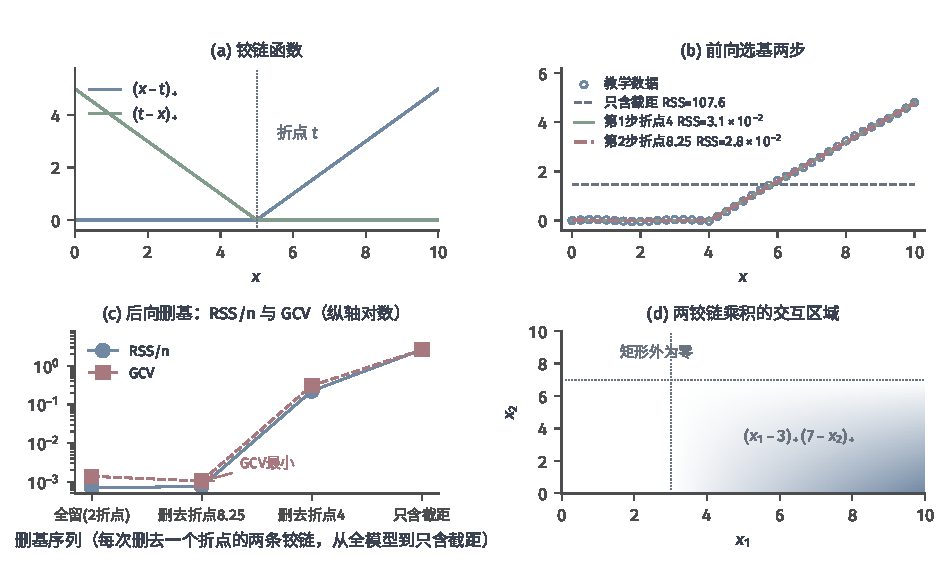
\includegraphics[width=159.0mm]{figures/07-classic-models/00-shared/matplotlib/regression-mars-mechanism/figure.pdf}
  \caption{MARS机制教学例（确定性一维构造）。(a)铰链$(x-t)_+$与$(t-x)_+$在折点$t$处连续、外侧一侧为零；(b)前向两步：空心圆点为教学数据，每步在样本位置处成对加入铰链，按真实最小二乘RSS下降最大者挑选；绿色实线为第1步（折点4）、红色点划线为第2步（再加折点8.25），两线差别仅在小波纹处，图例给出各步RSS；(c)后向删基（纵轴对数）：RSS/n随删基单调上升，GCV在删去折点8.25处最低（已标注）——多出的折点只换来微小RSS改善，折点惩罚使其不划算；(d)两铰链乘积$(x_1-3)_+(7-x_2)_+$只在矩形$x_1>3,\ x_2<7$内非零。数据为解析式教学构造（单折点分段线性目标加固定小波纹），非真实实验。}
  \label{fig:regression-mars-mechanism}
\end{figure*}

\subsubsection{性质与限制}
\label{sec:regression-mars-theory}

铰链$(x-t)_+$及其乘积在折点处连续但不可导，因此MARS展开整体连续、分段线性，交互阶数与单变量结点数量不是同一能力。外推到训练域外时，铰链项要么归零、要么线性增长，观测之外的走势不保证合理，需要独立验证。

前向选基是贪心：每步只选当前下降最多的项，不保证全局最优子集。GCV只是留一误差的近似，折点在全部样本位置中搜索、候选枚举与逐折重估本身也有计算代价，规模序列较长时实现上需控制候选范围。

\paragraph{与相邻方法对照}

与回归树对照：树的指示函数是硬划分，落入叶内用常数；MARS用连续铰链替代硬开关，在折点两侧平滑过渡。与固定基函数回归对照：两者都是基上的线性展开，差别在于基由人工指定还是由数据选择，后者把选基本身变成了学习问题。
